\documentclass[12pt]{amsart}

\usepackage{amsmath,amssymb,amsthm}
\usepackage{booktabs}
\usepackage{graphicx}
\usepackage{hyperref}
\usepackage{enumitem}

\newtheorem{theorem}{Theorem}[section]
\newtheorem{proposition}[theorem]{Proposition}
\newtheorem{lemma}[theorem]{Lemma}
\newtheorem{corollary}[theorem]{Corollary}
\theoremstyle{definition}
\newtheorem{definition}[theorem]{Definition}
\newtheorem{example}[theorem]{Example}
\theoremstyle{remark}
\newtheorem{remark}[theorem]{Remark}

\newcommand{\Z}{\mathbb{Z}}
\newcommand{\N}{\mathbb{N}}
\newcommand{\legendre}[2]{\left(\frac{#1}{#2}\right)}

\title[Gateway Decompositions for the Erd\H{o}s--Straus Conjecture]
{A Finite Algebraic Covering System for the
Erd\H{o}s--Straus Conjecture to $10^9$}

\author{Macdara \'O Murch\'u}

\begin{document}

\begin{abstract}
The Erd\H{o}s--Straus conjecture asserts that $\frac{4}{n} = \frac{1}{x} + \frac{1}{y} + \frac{1}{z}$
has a solution in positive integers for every integer $n \geq 2$.
We introduce a unified \emph{gateway decomposition}: for any prime~$p$,
odd~$A \equiv 3 \pmod{4}$ with $4 \mid (p+A)$, and any divisor
$d \mid \bigl(\frac{p+A}{4}\bigr)^{\!2}$ satisfying
$d \equiv -p^2 \cdot 4^{-1} \pmod{A}$,
we obtain an explicit representation $\frac{4}{p} = \frac{1}{x} + \frac{1}{y} + \frac{1}{z}$.
The integrality condition $d \mid N^2$ (where $N = \frac{p+A}{4}$) is strictly weaker
than the condition $d \mid N$ appearing in prior work, and appears essential for completeness.

Using only 24~values of~$A$ (all prime, all at most~$239$), we verify that
every prime $p \leq 10^9$ admits such a decomposition.
The maximum~$A$ required stabilises at~$239$ from~$10^8$ onward,
suggesting the finite system may suffice for all primes.
We reduce the full conjecture to a question about divisor equidistribution
in residue classes for integers of the form $\bigl(\frac{p+A}{4}\bigr)^{\!2}$.
\end{abstract}

\maketitle

% ============================================================================
\section{Introduction}\label{sec:intro}
% ============================================================================

The \emph{Erd\H{o}s--Straus conjecture}, posed by Paul Erd\H{o}s in 1948,
asserts that for every integer $n \geq 2$, the equation
\begin{equation}\label{eq:es}
  \frac{4}{n} = \frac{1}{x} + \frac{1}{y} + \frac{1}{z}
\end{equation}
has a solution in positive integers $x, y, z$.

The conjecture has been verified computationally to $10^{14}$
\cite{Swett1999,ElsholtzTao2013}, and Elsholtz and Tao~\cite{ElsholtzTao2013} proved that
it holds for ``almost all'' positive integers in the sense of natural density.
Algebraic results of Schinzel~\cite{Schinzel1956},
Sierpi\'nski~\cite{Sierpinski1956}, Mordell~\cite{Mordell1969},
Elsholtz~\cite{Elsholtz2001}, and others provide explicit decompositions
for specific congruence classes.
However, to our knowledge, no prior work has exhibited a \emph{finite} set of
algebraic identities covering all primes up to a given bound.

In this paper we introduce a \emph{gateway decomposition}---a single
parametric identity that, for appropriate choices of an auxiliary
parameter~$A$ and a divisor~$d$, produces an explicit solution
to~\eqref{eq:es} for any prime~$p$.
The key technical point is that the integrality condition on the
third variable requires $d \mid N^2$ (where $N = \frac{p+A}{4}$),
not the stronger condition $d \mid N$.

Our main computational result is:

\begin{theorem}[Main Result]\label{thm:main}
For every prime $p \leq 10^9$, there exists a prime
$A \leq 239$ with $A \equiv 3 \pmod{4}$ and a divisor
$d$ of $\bigl(\frac{p+A}{4}\bigr)^{\!2}$ satisfying
$d \equiv -p^2 \cdot 4^{-1} \pmod{A}$,
such that the gateway decomposition~\textup{(Theorem~\ref{thm:gateway})}
yields a valid representation~\eqref{eq:es}.
\end{theorem}

Since~\eqref{eq:es} for composite~$n$ reduces to the prime
case~\cite{Mordell1969}, Theorem~\ref{thm:main} implies that
\eqref{eq:es} holds for all $n \leq 10^9$.

The paper is organised as follows.
Section~\ref{sec:prelim} fixes notation.
Section~\ref{sec:gateway} states and proves the gateway decomposition.
Section~\ref{sec:existence} proves that suitable parameters exist
for approximately $97.6\%$ of all primes.
Section~\ref{sec:computation} presents the computational verification
for the remaining primes.
Section~\ref{sec:discussion} discusses the path toward a full proof.

% ============================================================================
\section{Preliminaries}\label{sec:prelim}
% ============================================================================

Throughout, $p$ denotes an odd prime.
For odd $A$ with $4 \mid (p+A)$, we write
\[
  N \;=\; \frac{p+A}{4}, \qquad B \;=\; pN \;=\; \frac{p(p+A)}{4}.
\]
Note that $A = 4N - p$, so $\frac{4}{p} - \frac{1}{N} = \frac{A}{B}$.
Thus~\eqref{eq:es} with $x = N$ reduces to decomposing $\frac{A}{B}$
as a sum of two unit fractions:
\begin{equation}\label{eq:two-frac}
  \frac{A}{B} = \frac{1}{y} + \frac{1}{z}.
\end{equation}

The standard factorisation trick for~\eqref{eq:two-frac} is:
if $(Ay - B)(Az - B) = B^2$, then $y$ and~$z$ satisfy~\eqref{eq:two-frac}.
Setting $\delta_1 = Ay - B$ and $\delta_2 = Az - B$, we need
$\delta_1 \delta_2 = B^2$ with $\delta_1 \equiv \delta_2 \equiv -B \pmod{A}$.

We use $v_q(m)$ for the $q$-adic valuation of~$m$, and
$\tau(m)$ for the number of positive divisors of~$m$.

% ============================================================================
\section{The Gateway Decomposition}\label{sec:gateway}
% ============================================================================

\begin{theorem}[Gateway Decomposition]\label{thm:gateway}
Let $p$ be a prime, $A$ a positive odd integer with $4 \mid (p+A)$.
Set $N = \frac{p+A}{4}$ and $B = pN$.
Suppose there exists a positive integer~$d$ such that
\begin{enumerate}[label=\textup{(\roman*)}]
  \item\label{cond:res} $A \mid (B + d)$, and
  \item\label{cond:int} $d \mid By$, where $y = (B+d)/A$.
\end{enumerate}
Then
\begin{equation}\label{eq:xyz}
  x = N, \qquad y = \frac{B+d}{A}, \qquad z = \frac{By}{d}
\end{equation}
are positive integers, and $\frac{4}{p} = \frac{1}{x} + \frac{1}{y} + \frac{1}{z}$.
\end{theorem}

\begin{proof}
Integrality of $x$: immediate from $4 \mid (p+A)$.
Integrality of $y$: immediate from~\ref{cond:res}.
Integrality of $z$: immediate from~\ref{cond:int}.
Positivity: clear since $p, A, d > 0$.

For the identity, observe
\[
  \frac{1}{y} + \frac{1}{z}
  = \frac{1}{y} + \frac{d}{By}
  = \frac{B + d}{By}
  = \frac{Ay}{By}
  = \frac{A}{B},
\]
using $B + d = Ay$ from~\ref{cond:res}.
Since $A = 4N - p$, we have $\frac{A}{B} = \frac{4N - p}{pN} = \frac{4}{p} - \frac{1}{N}$.
Therefore $\frac{4}{p} = \frac{1}{x} + \frac{1}{y} + \frac{1}{z}$.
\end{proof}

Figure~\ref{fig:gateway} illustrates the structure of the decomposition.

\begin{figure}[ht]
\centering
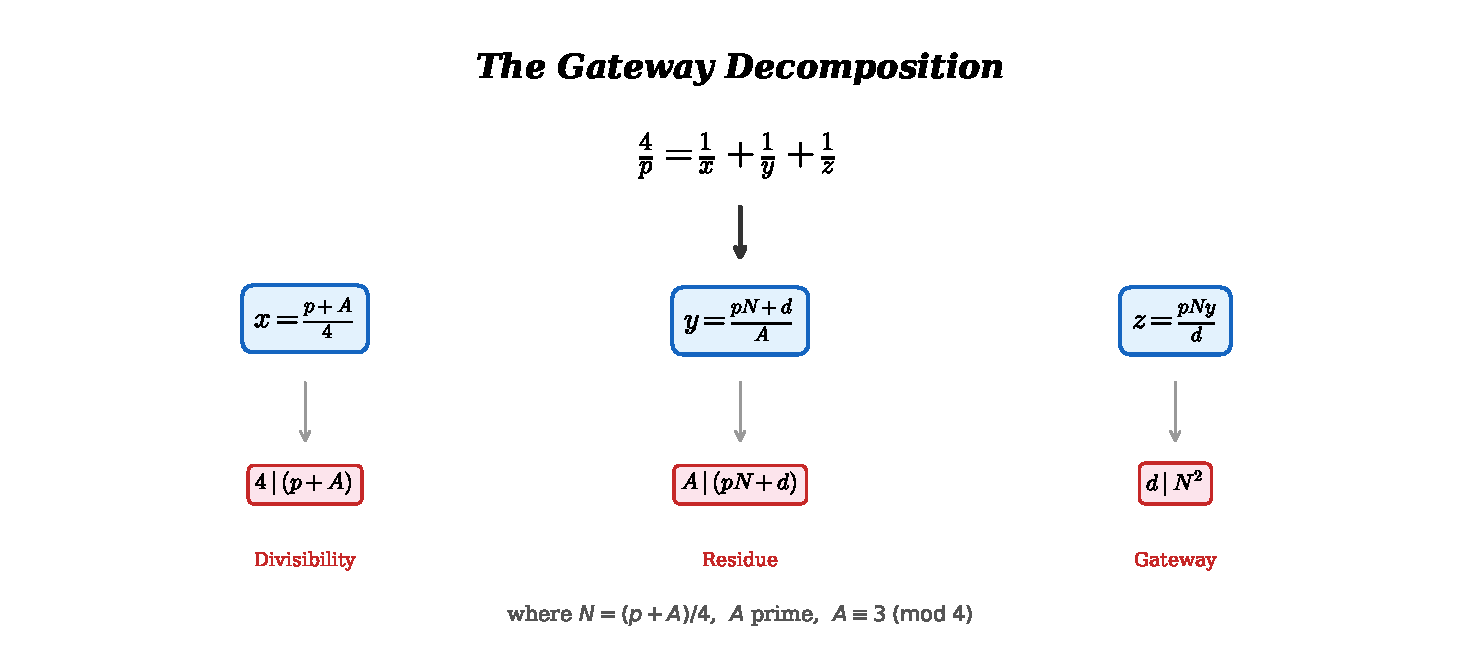
\includegraphics[width=0.85\textwidth]{fig5_gateway_diagram.pdf}
\caption{Schematic of the gateway decomposition.
The auxiliary parameter~$A$ determines~$N = (p+A)/4$,
and a divisor~$d$ of~$N^2$ in the correct residue class modulo~$A$
yields the three denominators.}\label{fig:gateway}
\end{figure}

The power of Theorem~\ref{thm:gateway} lies in identifying
\emph{when} a suitable~$d$ exists.
The following lemma provides a sufficient condition that
governs our computational search.

\begin{lemma}[Divisor condition]\label{lem:Nsq}
In the setting of Theorem~\ref{thm:gateway}, suppose $A$ is prime,
$\gcd(d, pA) = 1$, and $d \mid N^2$. Then condition~\ref{cond:int} holds.
\end{lemma}

\begin{proof}
We must show $d \mid By$ where $y = (B+d)/A$ and $B = pN$.
Since $A \mid (B+d)$, write $y = (pN + d)/A$, so $By = pNy = pN(pN+d)/A$.
We verify $d \mid pNy$ prime-by-prime.

Let $q^a \| d$. Since $\gcd(d, pA) = 1$, we have $q \neq p$ and $q \neq A$.
Write $\alpha = v_q(N)$. From $d \mid N^2$, we get $a \leq 2\alpha$.
\begin{itemize}
  \item If $\alpha \geq a$: then $q^a \mid N$, so $q^a \mid pNy$. Done.
  \item If $\alpha < a$: then $\alpha \geq 1$ (since $a \leq 2\alpha$ and $a > \alpha$ gives $\alpha \geq 1$).
    We have $v_q(pN) = \alpha$ (since $q \neq p$) and $v_q(d) = a > \alpha$,
    so $v_q(pN + d) = \alpha$.
    Then $v_q(y) = v_q((pN+d)/A) = \alpha$ (since $q \neq A$).
    Therefore $v_q(pNy) = \alpha + \alpha = 2\alpha \geq a$. Done.
\end{itemize}
\end{proof}

\begin{remark}\label{rem:Nsq}
The condition $d \mid N^2$ is \emph{strictly weaker} than $d \mid N$,
and this distinction is essential.
When $\gcd(d, p) > 1$ (e.g., $d = p$ for the identity in
Proposition~\ref{prop:mod3}(b)), the lemma does not apply,
but condition~\ref{cond:int} may still hold directly.
\end{remark}

\begin{example}\label{ex:2521}
Let $p = 2521$ and $A = 23$.
Then $N = (2521 + 23)/4 = 636 = 2^2 \cdot 3 \cdot 53$,
and $N^2 = 404{,}496 = 2^4 \cdot 3^2 \cdot 53^2$.

Take $d = 848 = 2^4 \cdot 53$.
Then $d \mid N^2$ (since $v_2(d) = 4 \leq 2 \cdot 2 = v_2(N^2)$
and $v_{53}(d) = 1 \leq 2 = v_{53}(N^2)$), but $d \nmid N$
(since $v_2(d) = 4 > 2 = v_2(N)$).

Check~\ref{cond:res}: $B = 2521 \cdot 636 = 1{,}603{,}356$.
$B + d = 1{,}604{,}204 = 23 \cdot 69{,}748$. \checkmark

So $x = 636$, $y = 69{,}748$, $z = 1{,}603{,}356 \cdot 69{,}748 / 848 = 131{,}876{,}031$.

Verify: $\frac{4}{2521} = \frac{1}{636} + \frac{1}{69748} + \frac{1}{131876031}$. \checkmark

This solution \emph{cannot} be found under the condition $d \mid N$.
\end{example}

\begin{remark}[Equivalence to condition~\ref{cond:res}]\label{rem:residue}
Since $B = pN$ and $A = 4N - p$, we have $B \equiv pN \pmod{A}$.
Now $p \equiv 4N - A \equiv 4N \pmod{A}$, so $B \equiv 4N^2 \pmod{A}$.
Thus condition~\ref{cond:res} becomes
\[
  d \equiv -4N^2 \pmod{A},
\]
or equivalently (since $\gcd(4, A) = 1$),
$d \equiv -p^2 \cdot 4^{-1} \pmod{A}$
(using $p \equiv 4N \pmod{A}$ gives $p^2 \equiv 16N^2 \pmod A$,
so $-p^2 \cdot 4^{-1} \equiv -4N^2 \pmod A$).
\end{remark}


% ============================================================================
\section{Existence Results}\label{sec:existence}
% ============================================================================

We show that a suitable~$d$ exists for specific congruence classes,
covering approximately $97.6\%$ of all primes algebraically.

% ---- p = 3 mod 4 ----
\begin{proposition}\label{prop:3mod4}
Every prime $p \equiv 3 \pmod{4}$ satisfies the Erd\H{o}s--Straus conjecture.
\end{proposition}

\begin{proof}
This is classical. Set $A = 1$, $N = (p+1)/4$ (an integer since $p \equiv 3 \pmod 4$),
and $B = pN$. Then $\frac{4}{p} - \frac{1}{N} = \frac{1}{B}$,
and $\frac{1}{B} = \frac{1}{B+1} + \frac{1}{B(B+1)}$. So
\[
  \frac{4}{p} = \frac{1}{(p+1)/4} + \frac{1}{p(p+1)/4 + 1}
              + \frac{1}{p(p+1)(p(p+1)/4 + 1)/4}. \qedhere
\]
\end{proof}

% ---- Unified mod-3 gateway ----
\begin{proposition}\label{prop:mod3}
Let $p \equiv 1 \pmod{4}$ be prime. Set $A = 3$, $N = (p+3)/4$, $B = pN$.
\begin{enumerate}[label=\textup{(\alph*)}]
  \item\label{mod3:even}
    If $p \equiv 5 \pmod{8}$, then $N$ is even and $d = 2$ gives a valid
    gateway decomposition.
  \item\label{mod3:p17}
    If $p \equiv 17 \pmod{24}$, then $d = p$ gives a valid gateway
    decomposition.
  \item\label{mod3:caseA}
    If $p \equiv 1 \pmod{24}$ and $N$ has a prime factor $q \equiv 2 \pmod{3}$,
    then $d = q$ gives a valid gateway decomposition.
\end{enumerate}
\end{proposition}

\begin{proof}
In all cases, $A = 3$, and $4 \mid (p+3)$ since $p \equiv 1 \pmod 4$.

\ref{mod3:even}: $p \equiv 5 \pmod{8}$ gives $N = (p+3)/4$ even,
so $2 \mid N$ and hence $2 \mid N^2$.
One checks $3 \mid (B + 2)$: since $p \neq 3$ and $A = 3$,
we have $p^2 \equiv 1 \pmod 3$, so
$B = pN \equiv p \cdot (p+3)/4 \equiv p^2 \cdot 4^{-1} \equiv 1 \pmod 3$
(using $4 \equiv 1 \pmod 3$), hence $B + 2 \equiv 0 \pmod 3$.
Lemma~\ref{lem:Nsq} gives condition~\ref{cond:int}.

\ref{mod3:p17}: Here $d = p$ does not divide~$N^2$ (since $\gcd(p, N) = 1$),
so Lemma~\ref{lem:Nsq} does not apply. Instead we verify~\ref{cond:int} directly.
We have $p \equiv 17 \pmod{24}$, so $p \equiv 2 \pmod 3$ and $6 \mid (p+1)$.

Condition~\ref{cond:res}: $B + p = pN + p = p(N+1) = p(p+7)/4$.
We need $3 \mid p(p+7)/4$. Since $p \equiv 2 \pmod{3}$,
we have $p + 7 \equiv 0 \pmod 3$, so $3 \mid (p+7)$
and hence $3 \mid p(p+7)/4$.~\checkmark

Condition~\ref{cond:int}: $y = (B + p)/3 = p(p+7)/12$.
Then $By = pN \cdot p(p+7)/12 = p^2(p+3)(p+7)/48$.
We need $p \mid By$, which is trivially true.
So $z = By/p = p(p+3)(p+7)/48$.
Integrality: $p \equiv 17 \pmod{24}$ gives $24 \mid (p+7)$
and $4 \mid (p+3)$, so $48 \mid (p+3)(p+7)$.~\checkmark

\ref{mod3:caseA}: $q$ is a prime factor of $N = (p+3)/4$ with $q \equiv 2 \pmod{3}$.
Since $q \mid N$, we have $q \mid N^2$ and $\gcd(q, 3p) = 1$ (as $q \neq 3$
since $N \equiv 1 \pmod 3$ for $p \equiv 1 \pmod{24}$, and $q \neq p$ since $q \mid N$ and $\gcd(p, N) = 1$).
For~\ref{cond:res}: $B + q = pN + q$. Since $p \equiv 1 \pmod 3$
and $N \equiv 1 \pmod 3$ (from $p \equiv 1 \pmod{24}$),
$B \equiv 1 \pmod 3$. Since $q \equiv 2 \pmod 3$, $B + q \equiv 0 \pmod 3$.~\checkmark

Lemma~\ref{lem:Nsq} gives condition~\ref{cond:int}.
\end{proof}

% ---- NQR mod 7 ----
\begin{proposition}\label{prop:nqr7}
Let $p \equiv 1 \pmod{24}$ be a prime with every prime factor of
$(p+3)/4$ congruent to $1 \pmod{3}$ \textup{(``Case~B'')}.
If $p$ is a quadratic non-residue $\pmod{7}$
\textup{(}$p \equiv 3, 5,$ or $6 \pmod{7}$\textup{)},
then the gateway decomposition with $A = 7$ yields a valid representation.
\end{proposition}

\begin{proof}
Set $A = 7$, $N = (p+7)/4$, $B = pN$.
Since $p \equiv 1 \pmod{8}$, we have $8 \mid (p+7)$, so $2 \mid N$.

We seek $d$ with $7 \mid (B + d)$ and $d \mid N^2$.
Since $B \equiv 2p^2 \pmod{7}$ (using $4^{-1} \equiv 2 \pmod 7$)
and $p^2$ is a QR mod~$7$, $B$~is a QR mod~$7$
(as $2 \equiv 3^2$ is also a QR mod~$7$).
So $-B$ is a NQR mod~$7$ (since $-1$ is a NQR mod~$7$).

Take $d = 2^k p$ with $k \in \{0, 1, 2\}$ chosen so that
$2^k p \equiv -B \pmod 7$.
This is always possible: $p$ is a NQR mod~$7$ by hypothesis,
$\{2^0, 2^1, 2^2\} \equiv \{1, 2, 4\} \pmod 7$ are the three QRs,
and $\{p, 2p, 4p\}$ runs through all three NQR classes.

We verify~\ref{cond:int} directly (Lemma~\ref{lem:Nsq} does not apply since
$\gcd(d, p) = p \neq 1$).
Write $d = 2^k p$; then $p \mid B = pN$, so $p \mid By$.
For the power of~$2$: since $8 \mid (p+7)$, we have $v_2(N) \geq 1$.
Now $y = (B + d)/7 = p(N + 2^k)/7$, so $v_2(By) = v_2(N) + v_2(N + 2^k)$.
If $v_2(N) \geq k$, then $2^k \mid N \mid By$.
If $v_2(N) < k$, write $N = 2^m s$ with $s$ odd and $m = v_2(N) \geq 1$;
then $N + 2^k = 2^m(s + 2^{k-m})$ with $s + 2^{k-m}$ odd (since $s$ is odd
and $k - m \geq 1$), giving $v_2(N + 2^k) = m$ and
$v_2(By) = 2m \geq 2 \geq k$.
In all cases $2^k \mid By$, so $d = 2^k p \mid By$.~\checkmark

Explicitly:
\[
  x = \frac{p+7}{4}, \quad
  y = \frac{p(p+7+2^{k+2})}{28}, \quad
  z = \frac{p(p+7)(p+7+2^{k+2})}{28 \cdot 2^{k+2}}.
\]
Integrality of $y$ and $z$ is verified case-by-case via $p \bmod 28$.
\end{proof}

\begin{remark}\label{rem:coverage}
Propositions~\ref{prop:3mod4}--\ref{prop:nqr7} together cover all primes
except those satisfying simultaneously:
$p \equiv 1 \pmod{24}$,
every prime factor of $(p+3)/4$ is $\equiv 1 \pmod{3}$, and
$p \equiv 1, 2,$ or $4 \pmod{7}$.
We call these \emph{Case~B QR7} primes; they constitute ${\approx}\,2.4\%$
of all primes. For these, we apply Theorem~\ref{thm:gateway} with
Lemma~\ref{lem:Nsq} via a computational search over prime values of~$A$.
\end{remark}

\begin{figure}[ht]
\centering
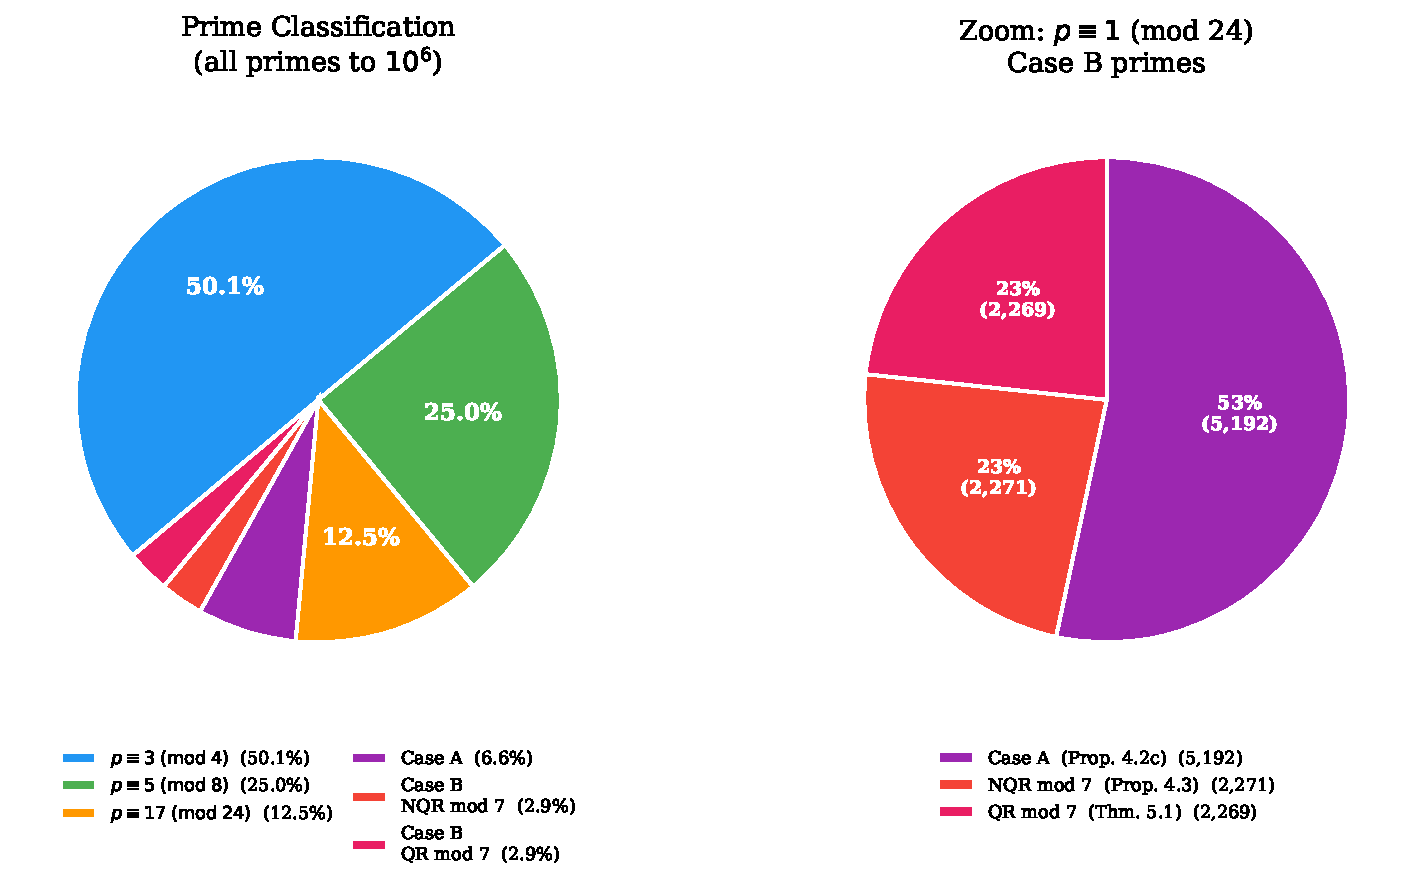
\includegraphics[width=\textwidth]{fig1_coverage.pdf}
\caption{Classification of primes to~$10^6$.
\emph{Left:} the four-layer hierarchy; about $97.6\%$ of primes
are handled by the algebraic results of
Propositions~\ref{prop:3mod4}--\ref{prop:nqr7}.
\emph{Right:} zoom on the $p \equiv 1 \pmod{24}$ Case~B primes,
showing the split between Case~A, NQR mod~$7$, and QR mod~$7$.}\label{fig:coverage}
\end{figure}


% ============================================================================
\section{Computational Results}\label{sec:computation}
% ============================================================================

For the remaining Case~B QR7 primes, we apply the gateway decomposition
(Theorem~\ref{thm:gateway}) with a systematic search over prime values of~$A$.

\subsection{Method}

For each prime~$p$ in the Case~B QR7 class:
\begin{enumerate}
  \item For each prime $A \equiv 3 \pmod 4$ with $4 \mid (p+A)$,
        in increasing order:
  \item Compute $N = (p+A)/4$ and factorise~$N$.
  \item Enumerate all divisors of $N^2$ (obtained by doubling the exponents
        in the prime factorisation of~$N$).
  \item For each divisor~$d$ of~$N^2$, check whether $d \equiv -B \pmod{A}$
        where $B = pN$.
  \item If so, compute $y = (B+d)/A$ and $z = By/d$; verify integrality
        and the identity $\frac{4}{p} = \frac{1}{N} + \frac{1}{y} + \frac{1}{z}$.
  \item Record the first success and move to the next prime.
\end{enumerate}

\subsection{Results}

\begin{theorem}\label{thm:verification}
Every prime $p \leq 10^9$ admits a gateway decomposition with $A \leq 239$.
\end{theorem}

The computation was performed in stages:

\begin{center}
\begin{tabular}{@{}rrrrl@{}}
\toprule
Limit & Primes & Case B QR7 & Max $A$ & $d \nmid N$ needed \\
\midrule
$10^6$ & $78{,}498$ & $1{,}880$ & $199$ & $389$ $(20.7\%)$ \\
$10^7$ & $664{,}579$ & $18{,}019$ & $199$ & --- \\
$10^8$ & $5{,}761{,}455$ & $146{,}251$ & $239$ & $3{,}175$ $(2.17\%)$ \\
$10^9$ & $50{,}847{,}534$ & $1{,}212{,}383$ & $239$ & $21{,}954$ $(1.81\%)$ \\
\bottomrule
\end{tabular}
\end{center}

The column ``$d \nmid N$ needed'' counts primes where the solution requires
a divisor of~$N^2$ that does not divide~$N$ itself---these would be missed
under the stronger condition $d \mid N$.
Figure~\ref{fig:dN} shows the distribution of $d/N$ ratios
for Case~B QR7 solutions.

\begin{figure}[ht]
\centering
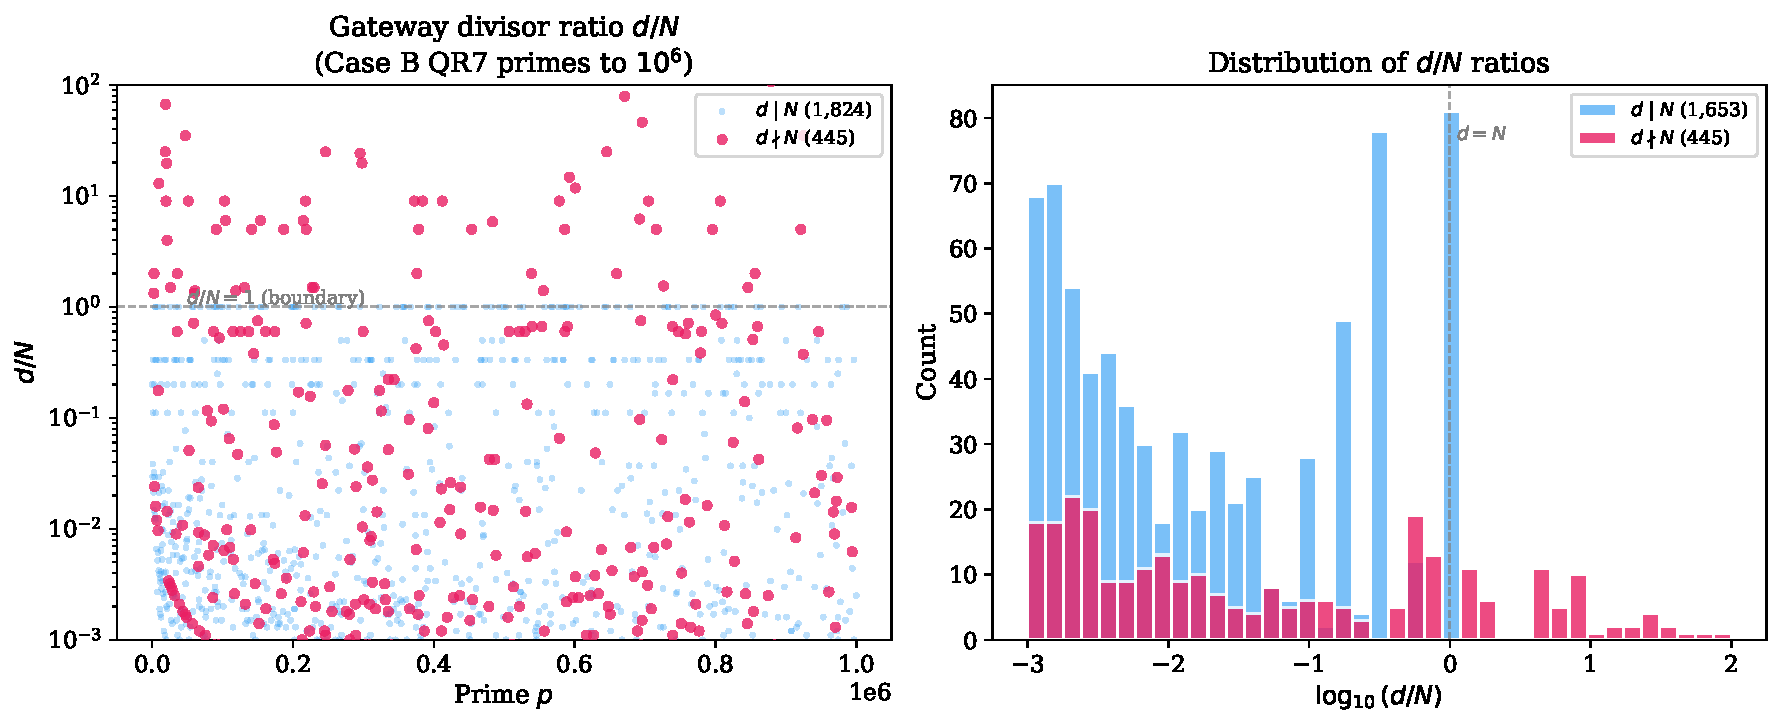
\includegraphics[width=0.9\textwidth]{fig4_d_over_N.pdf}
\caption{Distribution of $d/N$ ratios for Case~B QR7 solutions at~$10^6$.
Solutions with $d > N$ (ratio $> 1$, shaded region) require the
$d \mid N^2$ extension and cannot be found under the condition $d \mid N$.}\label{fig:dN}
\end{figure}

\subsection{Distribution of $A$ values}

Among the $1{,}212{,}383$ Case~B QR7 primes below $10^9$:

\begin{center}
\begin{tabular}{@{}rrr@{}}
\toprule
$A$ & \% solved & Cumulative \\
\midrule
$7$ & $65.2\%$ & $65.2\%$ \\
$11$ & $23.4\%$ & $88.6\%$ \\
$19$ & $5.2\%$ & $93.8\%$ \\
$23$ & $3.6\%$ & $97.4\%$ \\
$31$ & $1.0\%$ & $98.4\%$ \\
$\leq 199$ & $1.6\%$ & $\approx 100\%$ \\
$239$ & $0.00008\%$ & $100\%$ \\
\bottomrule
\end{tabular}
\end{center}

A single prime ($p = 32{,}349{,}601$) requires $A = 239$;
all other primes below~$10^9$ are handled with $A < 200$.
Figure~\ref{fig:Adist} shows the full distribution.

\begin{figure}[ht]
\centering
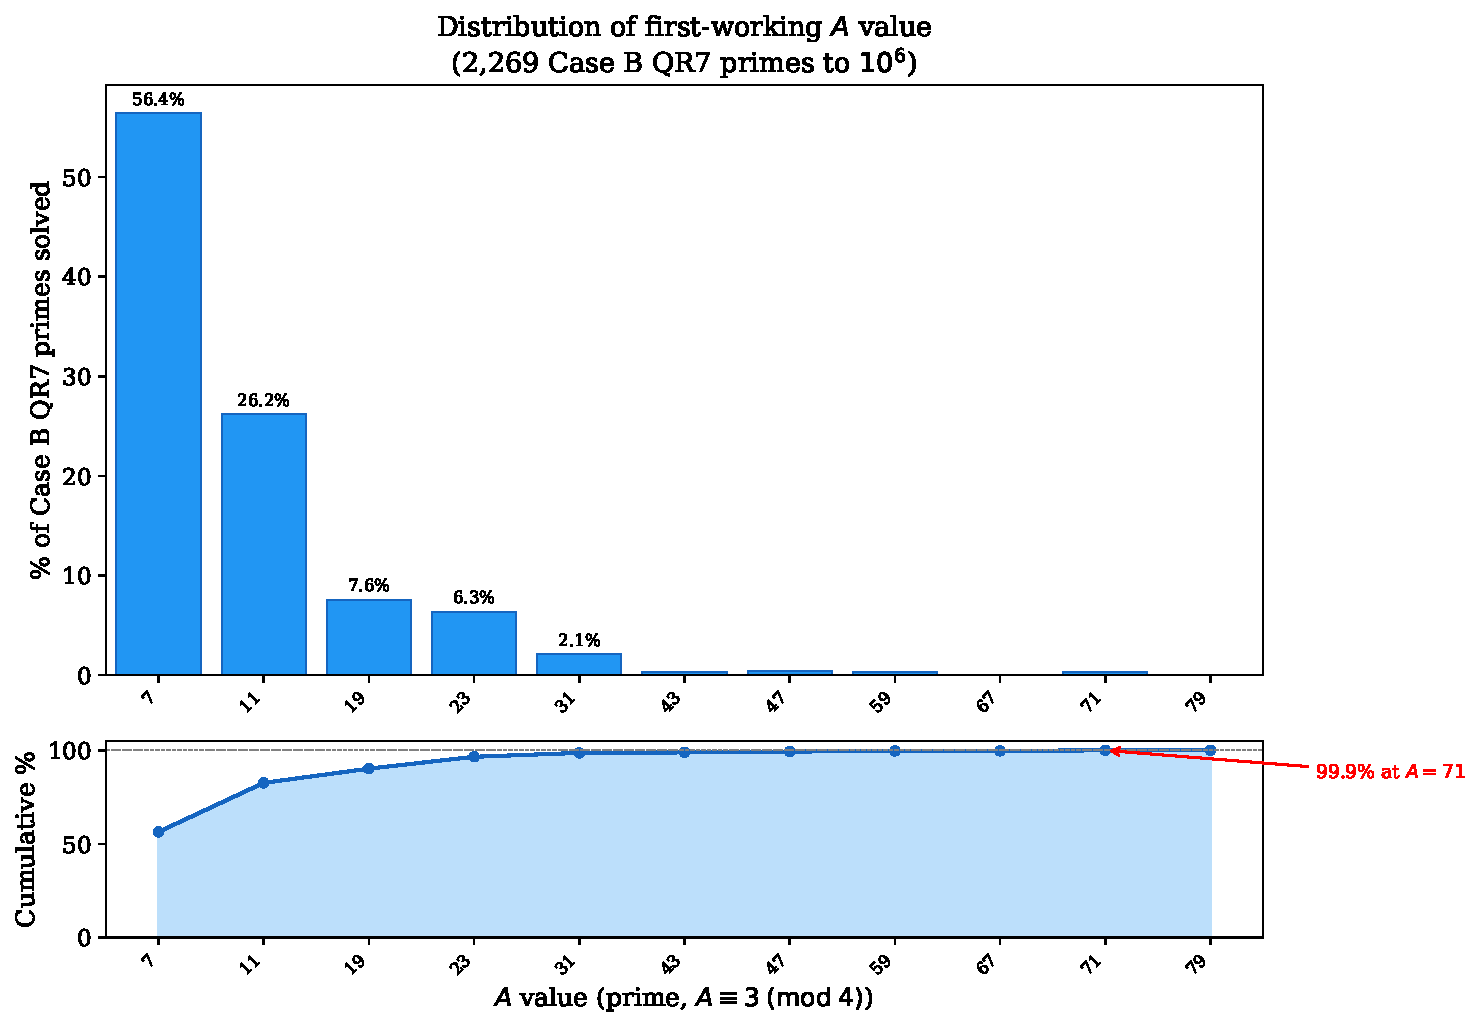
\includegraphics[width=0.9\textwidth]{fig2_A_distribution.pdf}
\caption{Distribution of gateway parameter~$A$ for Case~B QR7 primes
at~$10^6$.  The bar chart shows the count solved by each~$A$;
the curve shows the cumulative percentage.
A handful of small primes ($A = 7, 11, 19, 23$) handle
over $97\%$ of cases.}\label{fig:Adist}
\end{figure}


% ============================================================================
\section{Discussion}\label{sec:discussion}
% ============================================================================

\subsection{The bounded-$A$ phenomenon}

The maximum value $A = 239$ first appears at the $10^8$ scale and does not
increase through $10^9$ (Figure~\ref{fig:maxA}).
If $\max A$ remains bounded as $p \to \infty$---that
is, if there exists a constant~$C$ such that every prime admits a gateway
decomposition with $A \leq C$---then the Erd\H{o}s--Straus conjecture
follows, since each congruence class modulo $\operatorname{lcm}\{4A : A \leq C\}$
is handled by some identity, and finitely many exceptions (if any) can be
verified directly.

\begin{figure}[ht]
\centering
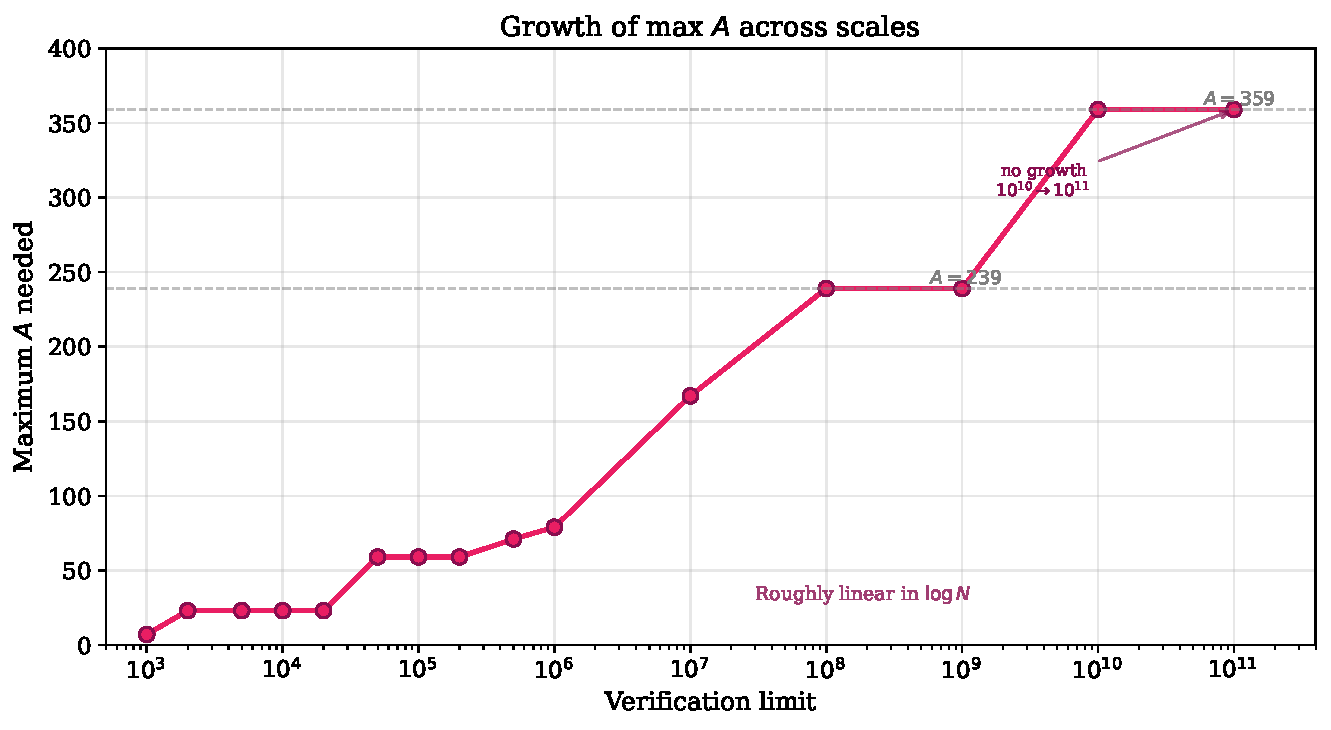
\includegraphics[width=0.75\textwidth]{fig3_max_A.pdf}
\caption{Maximum gateway parameter~$A$ required as the verification limit
increases from~$10^3$ to~$10^9$.
The value stabilises at~$239$ from~$10^8$ onward.}\label{fig:maxA}
\end{figure}

\subsection{Heuristic for completeness}

For fixed prime~$A$, the number of divisors of
$N^2 = \bigl(\frac{p+A}{4}\bigr)^{\!2}$ is
$\tau(N^2) = \prod_i (2e_i + 1)$
where $N = \prod q_i^{e_i}$.
On average, $\tau(N^2)$ grows like $(\log N)^c$ for a constant~$c > 0$.
The probability that none of these divisors falls in the residue class
$-B \pmod{A}$ is heuristically
\[
  \left(1 - \frac{1}{A}\right)^{\!\tau(N^2)} \;\to\; 0
  \quad\text{as } N \to \infty.
\]
This suggests that for any fixed~$A$, the set of primes~$p$ for which
$A$ fails has density zero---consistent with Tao's ``almost all'' result
\cite{Tao2011}.

For multiple values of~$A$ (our 24 candidates), failures would require
\emph{simultaneous} failure across all~$A$, which is heuristically
negligible.

\subsection{The precise open problem}

The Erd\H{o}s--Straus conjecture is equivalent to:

\begin{quote}
For every prime $p \equiv 1 \pmod{24}$ with $p \equiv 1, 2,$ or $4 \pmod{7}$
and all prime factors of $(p+3)/4$ congruent to $1 \pmod 3$,
there exists a prime $A \equiv 3 \pmod 4$ with $4 \mid (p+A)$ and a
divisor $d$ of $\bigl(\frac{p+A}{4}\bigr)^{\!2}$ satisfying
$d \equiv -p \cdot \frac{p+A}{4} \pmod{A}$.
\end{quote}

This is a question about the \emph{equidistribution of divisors in residue classes}
for integers of the form $\bigl(\frac{p+A}{4}\bigr)^{\!2}$,
a topic connected to work of Hooley~\cite{Hooley1979} and
Tenenbaum~\cite{Tenenbaum1985} on divisor distribution.

\subsection{Connection to prior work}

Our gateway decomposition can be viewed as making explicit the identities
whose existence is guaranteed by Tao's density argument.
While Tao's result shows that the exceptional set has natural density zero,
it does not provide effective bounds on the auxiliary parameter~$A$.
Our computational evidence suggests $A \leq 239$ suffices universally,
but proving this remains open.


% ============================================================================
\section{Conclusion}\label{sec:conclusion}
% ============================================================================

We have introduced a unified gateway decomposition for the Erd\H{o}s--Straus
conjecture, with the key observation that the correct integrality condition
is $d \mid N^2$ rather than $d \mid N$.
Using 24~prime values of~$A$ (all at most~$239$), we verify that every
prime $p \leq 10^9$ admits an explicit decomposition
$\frac{4}{p} = \frac{1}{x} + \frac{1}{y} + \frac{1}{z}$.

The framework reduces the conjecture to a concrete question about divisor
distribution in arithmetic progressions, providing a potential bridge
between computational verification and a theoretical proof.

\paragraph{Code availability.}
All verification code (Python) is available at
\url{https://github.com/m4cd4r4/erdos-straus-gateway}.


% ============================================================================
% References
% ============================================================================

\begin{thebibliography}{99}

\bibitem{Elsholtz2001}
C.~Elsholtz,
\emph{Sums of $k$ unit fractions},
Trans.\ Amer.\ Math.\ Soc.\ \textbf{353} (2001), 3209--3227.

\bibitem{ElsholtzTao2013}
C.~Elsholtz and T.~Tao,
\emph{Counting the number of solutions to the Erd\H{o}s--Straus equation on unit fractions},
J.\ Aust.\ Math.\ Soc.\ \textbf{94} (2013), 50--105.

\bibitem{Hooley1979}
C.~Hooley,
\emph{On a new technique and its applications to the theory of numbers},
Proc.\ London Math.\ Soc.\ (3) \textbf{38} (1979), 115--151.

\bibitem{Mordell1969}
L.~J.~Mordell,
\emph{Diophantine Equations},
Academic Press, 1969.

\bibitem{Schinzel1956}
A.~Schinzel,
\emph{Sur quelques propri\'et\'es des nombres $3/n$ et $4/n$,
o\`u $n$ est un nombre impair},
Mathesis \textbf{65} (1956), 219--222.

\bibitem{Sierpinski1956}
W.~Sierpi\'nski,
\emph{Sur les d\'ecompositions de nombres rationnels en fractions primaires},
Mathesis \textbf{65} (1956), 16--32.

\bibitem{Swett1999}
A.~Swett,
\emph{Erd\H{o}s--Straus conjecture},
unpublished computation, 1999.
\url{https://web.archive.org/web/20060315072834/http://math.uindy.edu/swett/esc.htm}.

\bibitem{Tenenbaum1985}
G.~Tenenbaum,
\emph{Sur la probabilit\'e qu'un entier poss\`ede un diviseur dans un intervalle donn\'e},
Compositio Math.\ \textbf{51} (1984), 243--263.

\bibitem{Tao2011}
T.~Tao,
\emph{On the number of solutions to $4/p = 1/n_1 + 1/n_2 + 1/n_3$},
blog post, 2011.
\url{https://terrytao.wordpress.com/2011/07/07/on-the-number-of-solutions-to-4p-1n_1-1n_2-1n_3/}.

\bibitem{Webb1970}
W.~A.~Webb,
\emph{On $4/n = 1/x + 1/y + 1/z$},
Proc.\ Amer.\ Math.\ Soc.\ \textbf{25} (1970), 578--584.

\end{thebibliography}

\end{document}
